

    %(Fill in bits about the squeezer)

Gravitational wave interferometry measures changes in light travel time far less than the light-crossing time of an atom, so the quantum nature of light has always influenced detector design.
Advanced LIGO aims to resolve most of noise sources described in Sections~\ref{methods} and~\ref{interferometer_theory}: even so, quantum shot and radiation pressure noise from light will remain.
Carlton Caves correctly derived the quantum behavior of interferometer shot and radiation pressure noise~\cite{Caves1980}.
Prior work had inferred the shot noise level from classical principles, accurately, but been ambiguous about radiation pressure.
With the quantum noise clarified, it was realized that this noise could be reduced through so-called squeezing of the vacuum state~\cite{Caves1981}.
This chapter describes part of how squeezing was successfully realized three decades later at the LIGO Hanford Observatory.
For additional details, consult Chua~\cite{ChuaThesis} and Dwyer~\cite{DwyerThesis}.

    \section{Squeezing theory}
    \label{squeezing_theory}

      %  Squeezing theory.
Quantum noise was initially treated as Poissonian photon counting (shot noise) and momentum coupling (radiation pressure), but it is better understood as the phase and amplitude uncertainty of the electromagnetic field at the interferometer output. 
Roughly speaking, phase uncertainty is equivalent to semi-classical shot noise and amplitude uncertainty to radiation pressure.
The standard quantum limit (SQL) on displacement sensitivity can be derived independently of either argument, as noted by Caves~\cite{Caves1981}:

\begin{equation}
(\Delta z)_{\textup{SQL}} = (2 \hbar \tau / m)^{1/2},
\label{sql_caves}
\end{equation}

\noindent where in Equation~\ref{sql_caves} $z$ is the mirror (test mass) displacement, $\tau$ is measurement duration, $\hbar$ is the reduced Planck constant, and $m$ is mirror mass.
When one tries to attain this standard quantum limit with an interferometer, then shot and radiation pressure are found to balance at a particular optimum input power $P_0$~\cite{Caves1981}:

\begin{equation}
P_0 = \frac{1}{2} \frac{mc^2}{\tau}\frac{1}{\omega \tau} \frac{1}{b^2},
\label{optimum_power_caves}
\end{equation}

\noindent with $\omega$ the angular frequency of light and $b$ the number of bounces (assuming delay lines, whereas a Fabry-Perot is proportional to finesse) in Equation~\ref{optimum_power_caves}.
The latter equation shows that the optimal power rises as $1/\sqrt{\tau}$, that is, as the squart root of the gravitational wave frequency.
Higher laser power improves high frequency sensitivity, high mirror mass improves low frequency performance.
Combined, these formulae imply that an interferometer should be built with the largest, most massive mirrors and most powerful lasers practicable.

LIGO and its allied interferometers do try to operate with massive optics and powerful lasers, but there are limits.
Vacuum enclosures place a constraint, only broken with significant expenditures, on the size of optical tables and mirror suspensions and therefore on mirror mass.
This indirectly limits laser power through the SQL.
Laser power, however, was not limited for this reason in initial and enhanced LIGO.
In practice, thermal distortion of the test masses was a worse problem~\cite{BallmerThesis}.
Absorption, both in the bulk of the fused silica substrate and in the HR coatings, of a few parts per million was sufficient to distort the radius of curvature of the Fabry-Perot cavities.
While managed with a $\textup{CO}_2$ laser-driven thermal compensation system (supplemented with ring heaters in aLIGO), this thermal distortion remains a serious concern.

Having an alternative to increased mirror size and laser power would grant flexibility.
Hence squeezing: the standard quantum limit can be achieved through another means.


        \subsection{Quantum shot noise and radiation pressure}
        \label{quantum_noise}

            %Carlton Caves, quantum shot noise and radiation pressure.

%\begin{frame}{Squeezing introduction}

%\begin{definition}
Altering $\Delta E\Delta\phi$ uncertainty for the electromagnetic
field
%\end{definition}
\begin{itemize}
\item Demonstrated first at GEO 600, then LIGO Hanford (H1)\end{itemize}
\begin{theorem}
Shot noise arises from quantum operators (Caves 1980, 1981)\end{theorem}
\begin{itemize}
\item Vacuum fluctuations couple through anti-symmetric port
\item \emph{Squeeze }the $\overrightarrow{E}$ field uncertainty ellipse
\item Angle $\theta$, factor $r$, creation operator $a$, squeeze operator
$S$:
\end{itemize}

From the Caves squeezing paper~\cite{Caves1981},

\[
S(\zeta)=\exp[\frac{1}{2}\zeta^{*}a^{2}-\frac{1}{2}\zeta(a^{\dagger})^{2}],\;\zeta=re^{i\theta}
\]



Squeezed state made with


optical parameter oscillator, 2nd harmonic generator


\textbf{Shot noise reduced by $e^{-r}$}


\[
\]




        \subsection{Problems with lasers: thermal compensation}
        \label{TCS}

            Experience (some firsthand) with thermal compensation.

        \subsection{Squeezing filter cavities against alternatives}
        \label{third-gen_squeezing}

    \section{LIGO Hanford Observatory quantum vacuum squeezing}
    \label{LHO_squeeze}

        Quantum vacuum squeezing at LIGO Hanford Observatory. Naturally, a great deal of description and background will come from Sheila Dwyer's thesis~\cite{DwyerThesis} and Sheon Chua's thesis~\cite{ChuaThesis}.

        \subsection{Collaboration and contributions}
        \label{contributions}

            Contributions: table, in-vacuum installation, electronics, range est.

            \subsubsection{Optical table support assembly}
            \label{table_legs}

                Table legs (me) and results of Sheon and Robert's shakers.

		Here might be good place to put old AutoCAD drawings to use.
\begin{figure}
\begin{center}
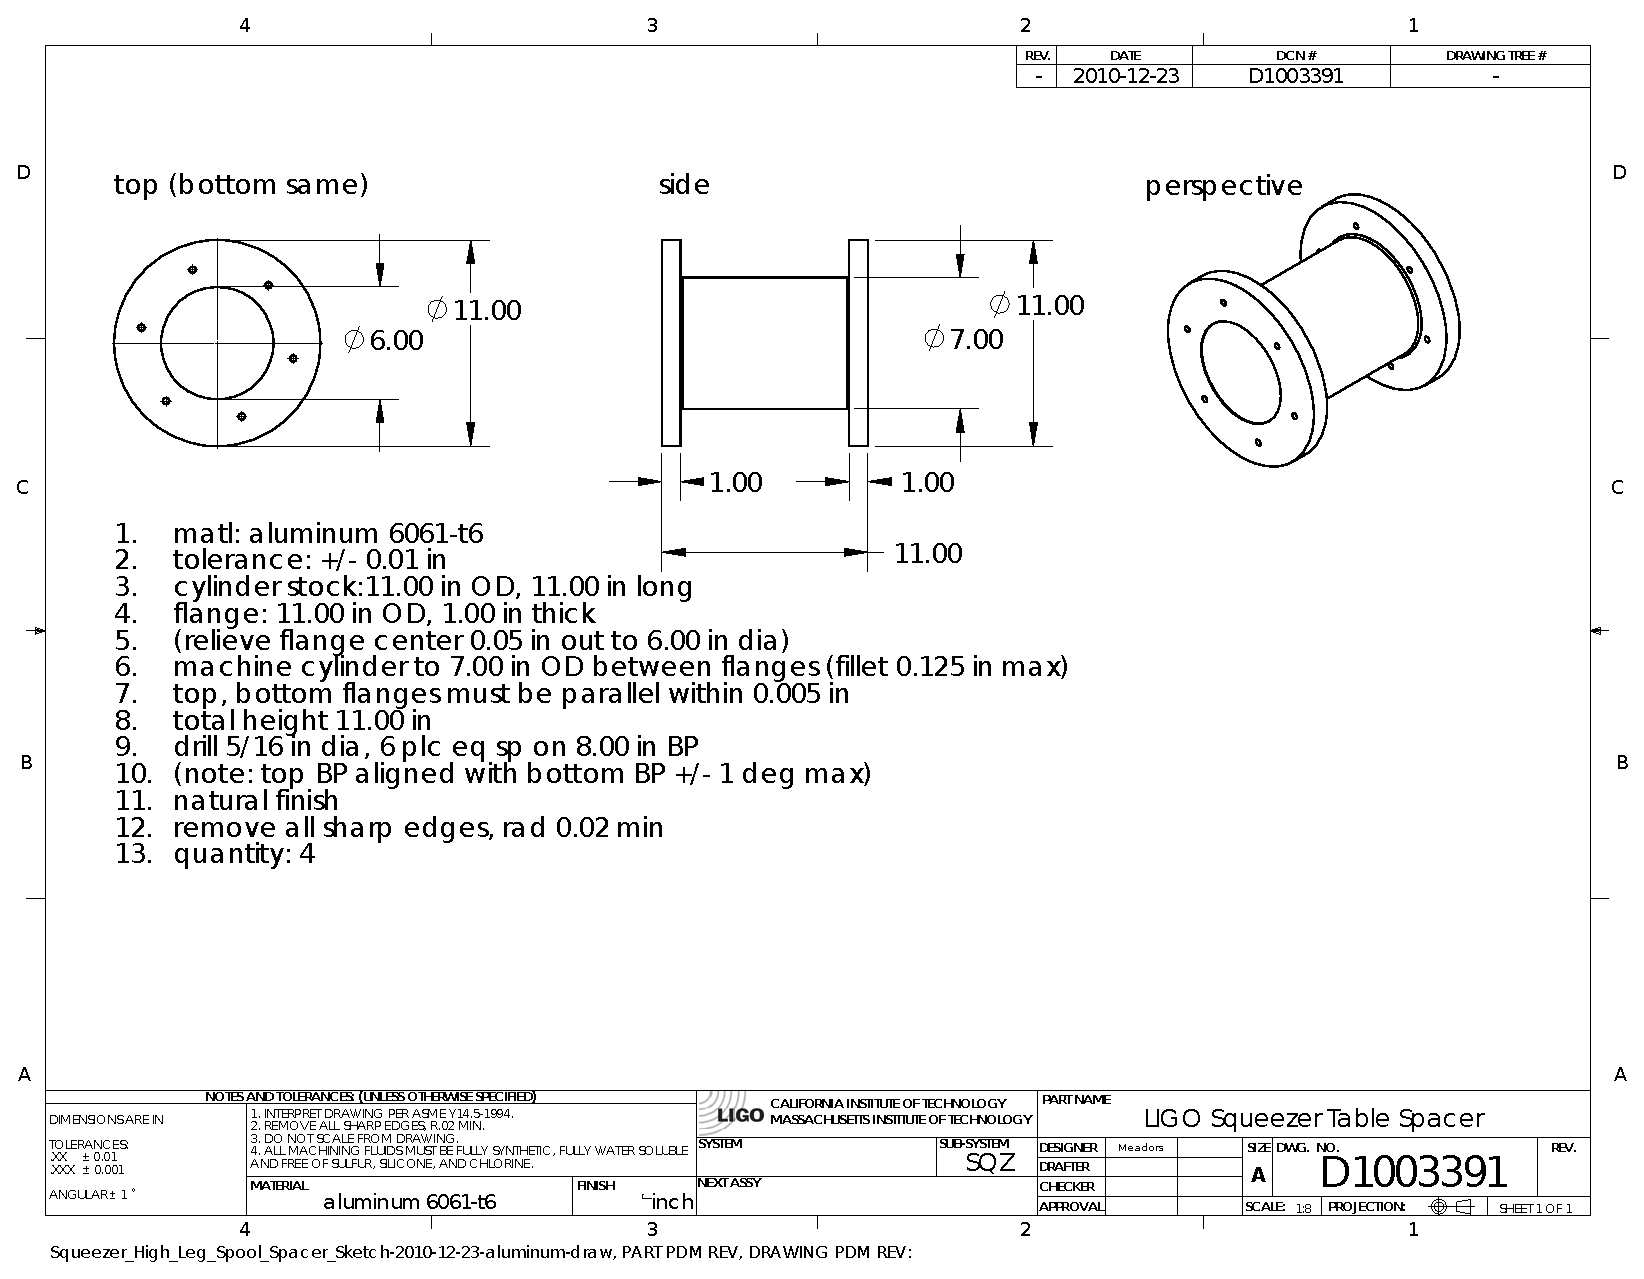
\includegraphics[width=0.6\paperwidth]{Squeezer_High_Leg_Spool_Spacer_2010-12-23_aluminum.eps}
\caption{Table legs SolidWorks schematic. This initial design for the table leg extensions on the squeezer table incorporated a flange, which was removed immediately prior to fabrication, replaced with a larger diameter flangeless tube with incorporated tap-holes. Flanges were thought necessary for a flexible alignment initially, they would be prohibitively expensive to machine, and welding would induce unacceptable distortions into the metal. Design in consultation with Daniel Sigg, Lisa Barsotti, Keita Kawabe, Gerardo Moreno, Richard Savage.
}
\end{center}
\end{figure}


            \subsubsection{Faraday isolator measurement}
            \label{Faraday}

                Faraday isolator measurements were performed by Keita Kawabe, Matt Evans, Lisa Barsotti along with myself.

		What were the results of the measurement? Show e-log entries, comment on in-and-out-of-vacuum performance and what it says about the need for low loss to be a top priority in future squeezing efforts.

            \subsubsection{In-vacuum installation}
            \label{In-vacuum}

                In-vacuum Faraday and baffle installation with "".

                Show pictures of the installation, connect to the issues with stray and perhaps backscattered light.

		Discuss the repair of the output mode cleaner, which is mentioned (citation 50) in Nic's thesis~\cite{SmithThesis}. The technical report corresponding to it is by Waldman and Chua~\cite{Waldman2011}.

            \subsubsection{Data digitization}
            \label{data_digitization}

                Electronic cabling and analog-to-digital converter installation.
                Added data channels with David Barker.

		May want helpful diagram.



%\end{frame}

%\begin{frame}{Squeezing large interferometers}


\begin{figure}
\begin{center}
%\protect\caption{\protect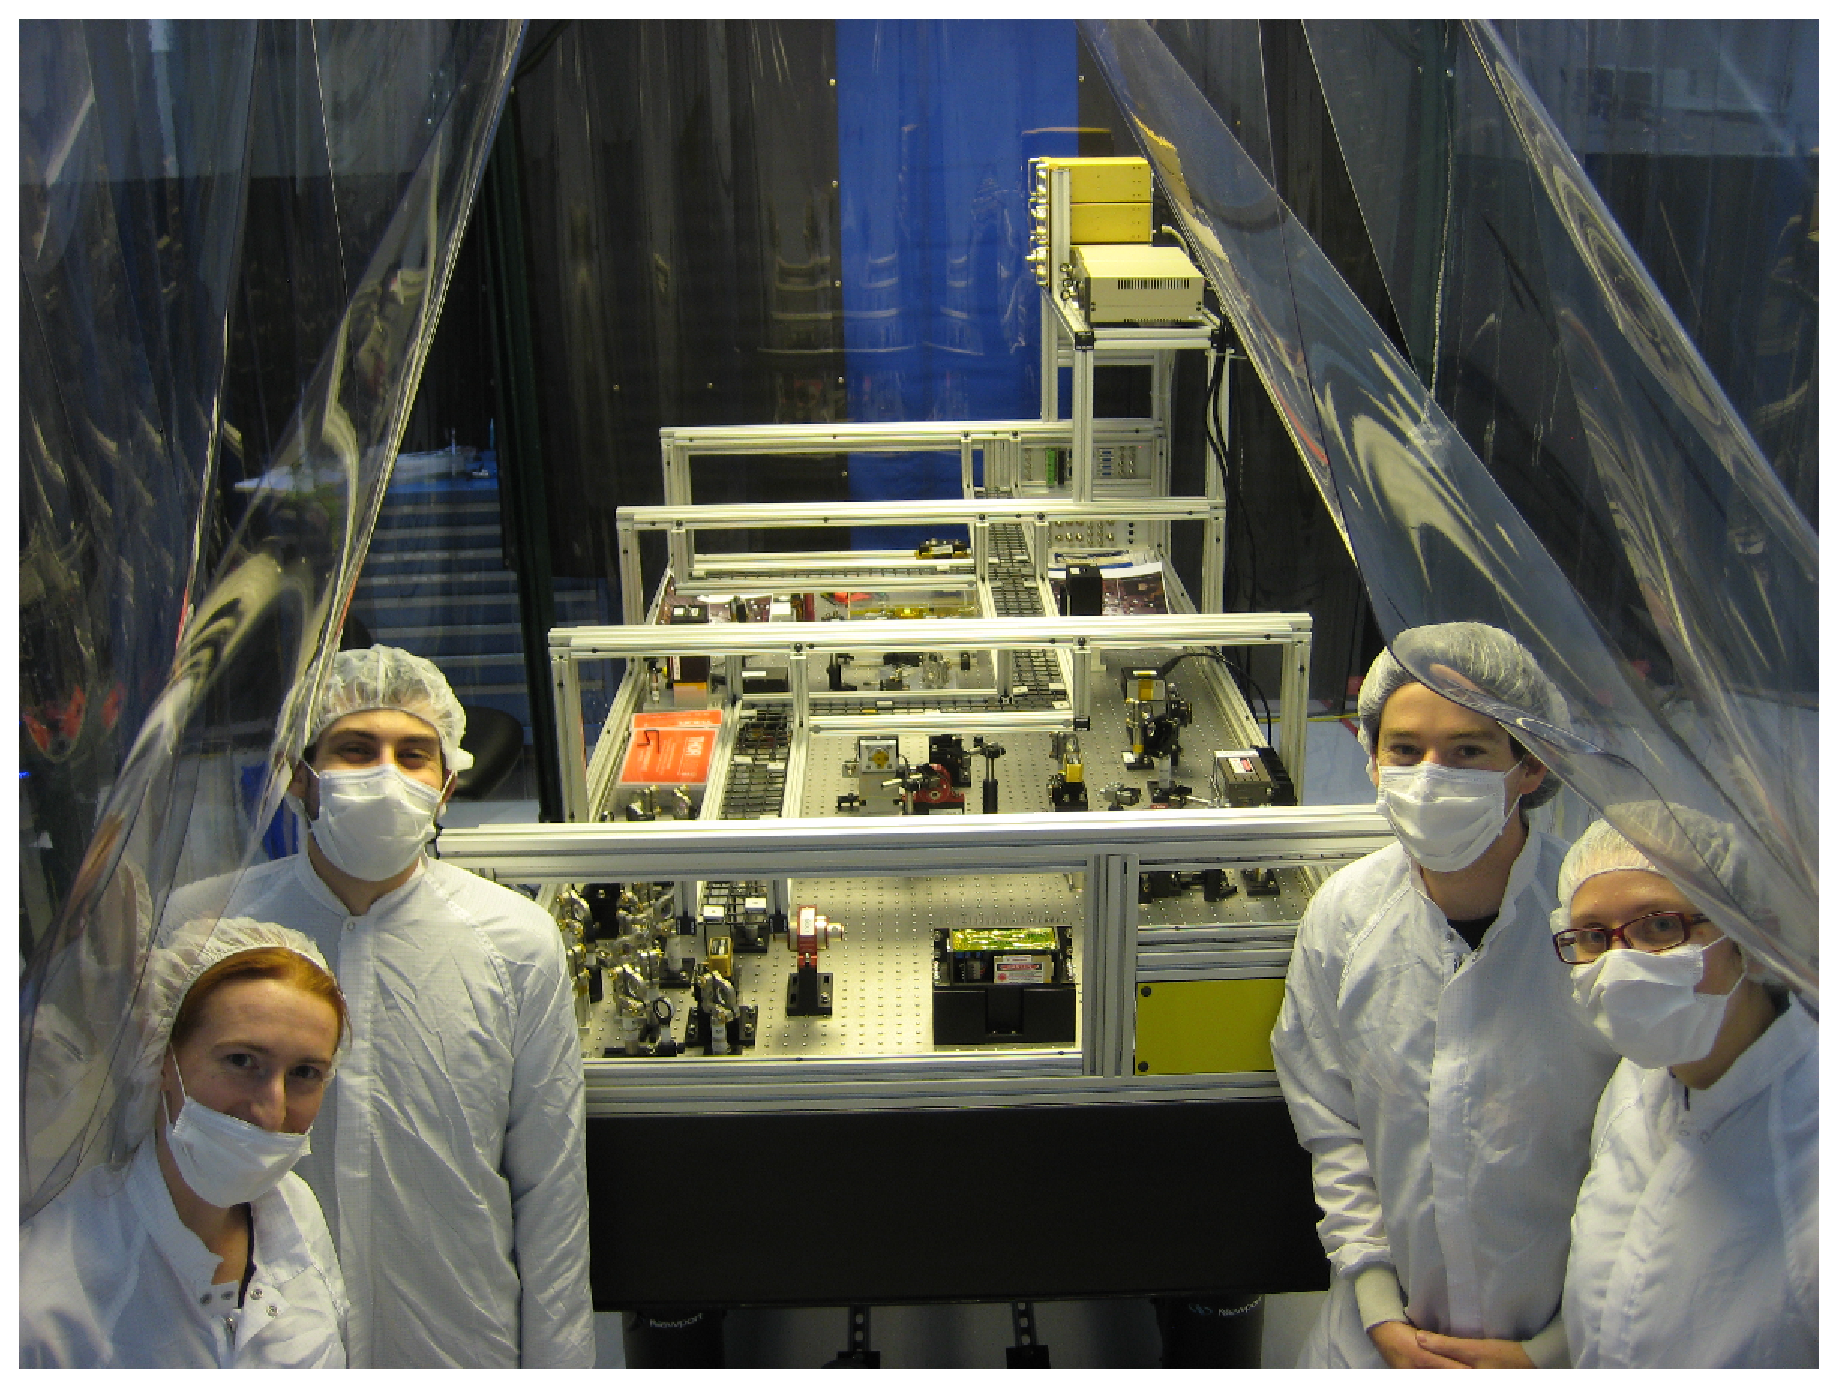
\includegraphics[width=0.33\paperwidth]{lisabar-1289966130}}
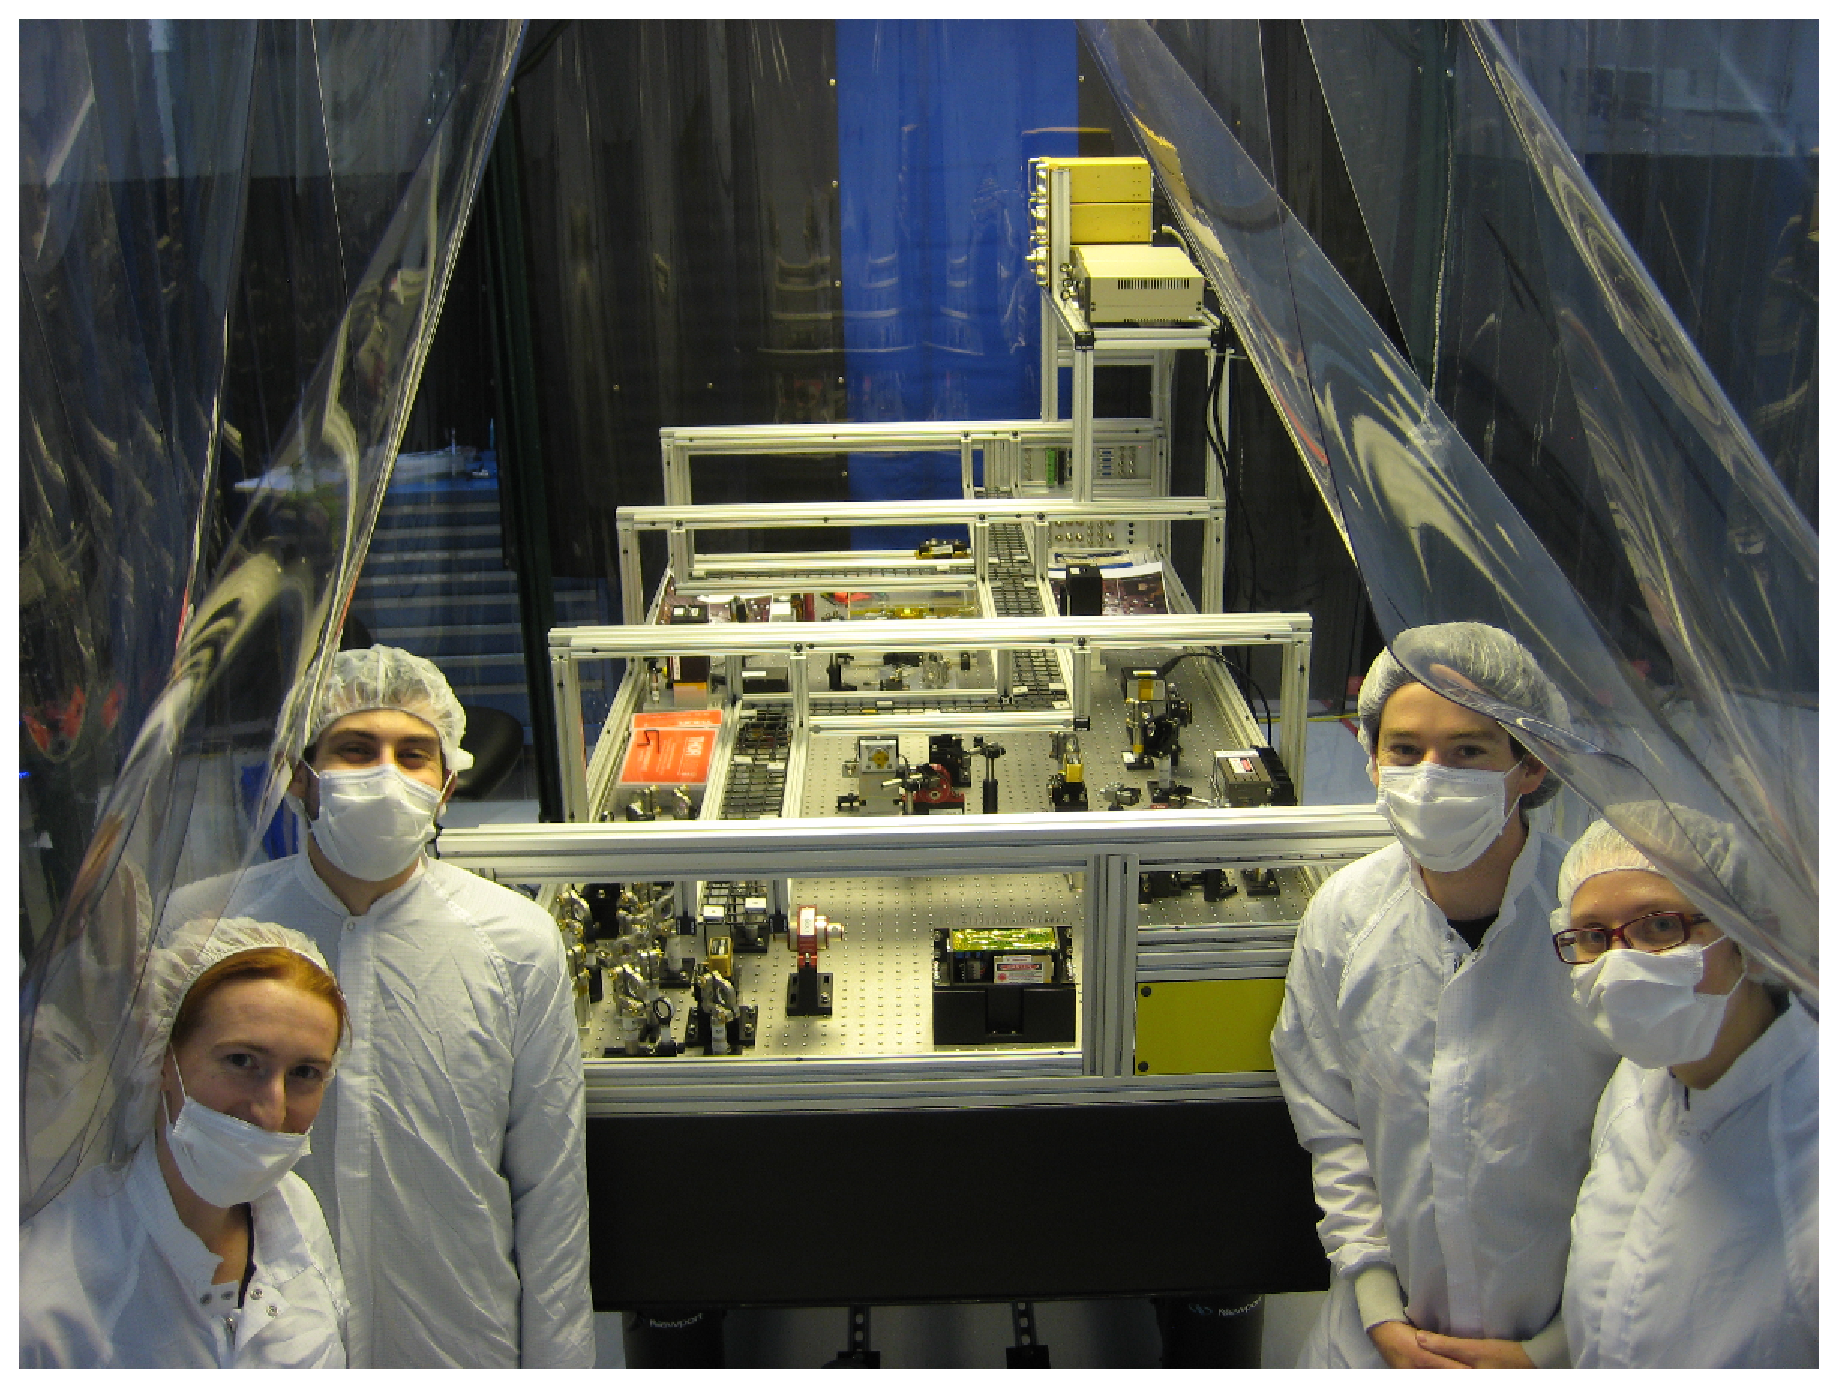
\includegraphics[width=0.6\paperwidth]{lisabar-1289966130.eps}


%\protect\caption{\protect\includegraphics[width=0.33\paperwidth]{lisabar-1300943141}}


\caption{Image by Lisa Barsotti in Hanford eLog.
\newline Counterclockise from lower left: Sheila Dwyer, Lisa Barsotti, Conor Mow-Lowry, Grant Meadors. This photograph shows the uncovered squeezer table with components from the MIT squeezer experiment unpacked at LIGO Hanford Observatory in November 2010. The table sat in a temporary location by HAM6, where it was recommissioned by Dwyer, Mow-Lowry, Sheon Chua, and Alexander Khalaidovksi until H1 could be brought back online for the squeezing experiment in late 2011. 
}
\end{center}
\end{figure}
\begin{figure}
\begin{center}
\includegraphics[width=0.6\paperwidth]{lisabar-1300943141.eps}
\caption{Table legs testing. The squeezer table is raised to its final height by the leg extensions. From top to bottom: table (WISCT10), existing leg extensions (with flanges), new leg extensions (flangeless), triangular high table legs. This assemblage provided the squeezer a serendiptously-stable (as measured by Sheila Dwyer and Robert Schoield) platform at low cost. Photo in temporary location; the actual squeezer table was anchored to these table legs, grouted, by HAM4.
}
\end{center}
\end{figure}


%\end{frame}

%\begin{frame}{Squeezing's scientific benefit}
\subsection{Squeezing's scientific benefit}


\begin{figure}
\begin{center}
%\protect\caption{\protect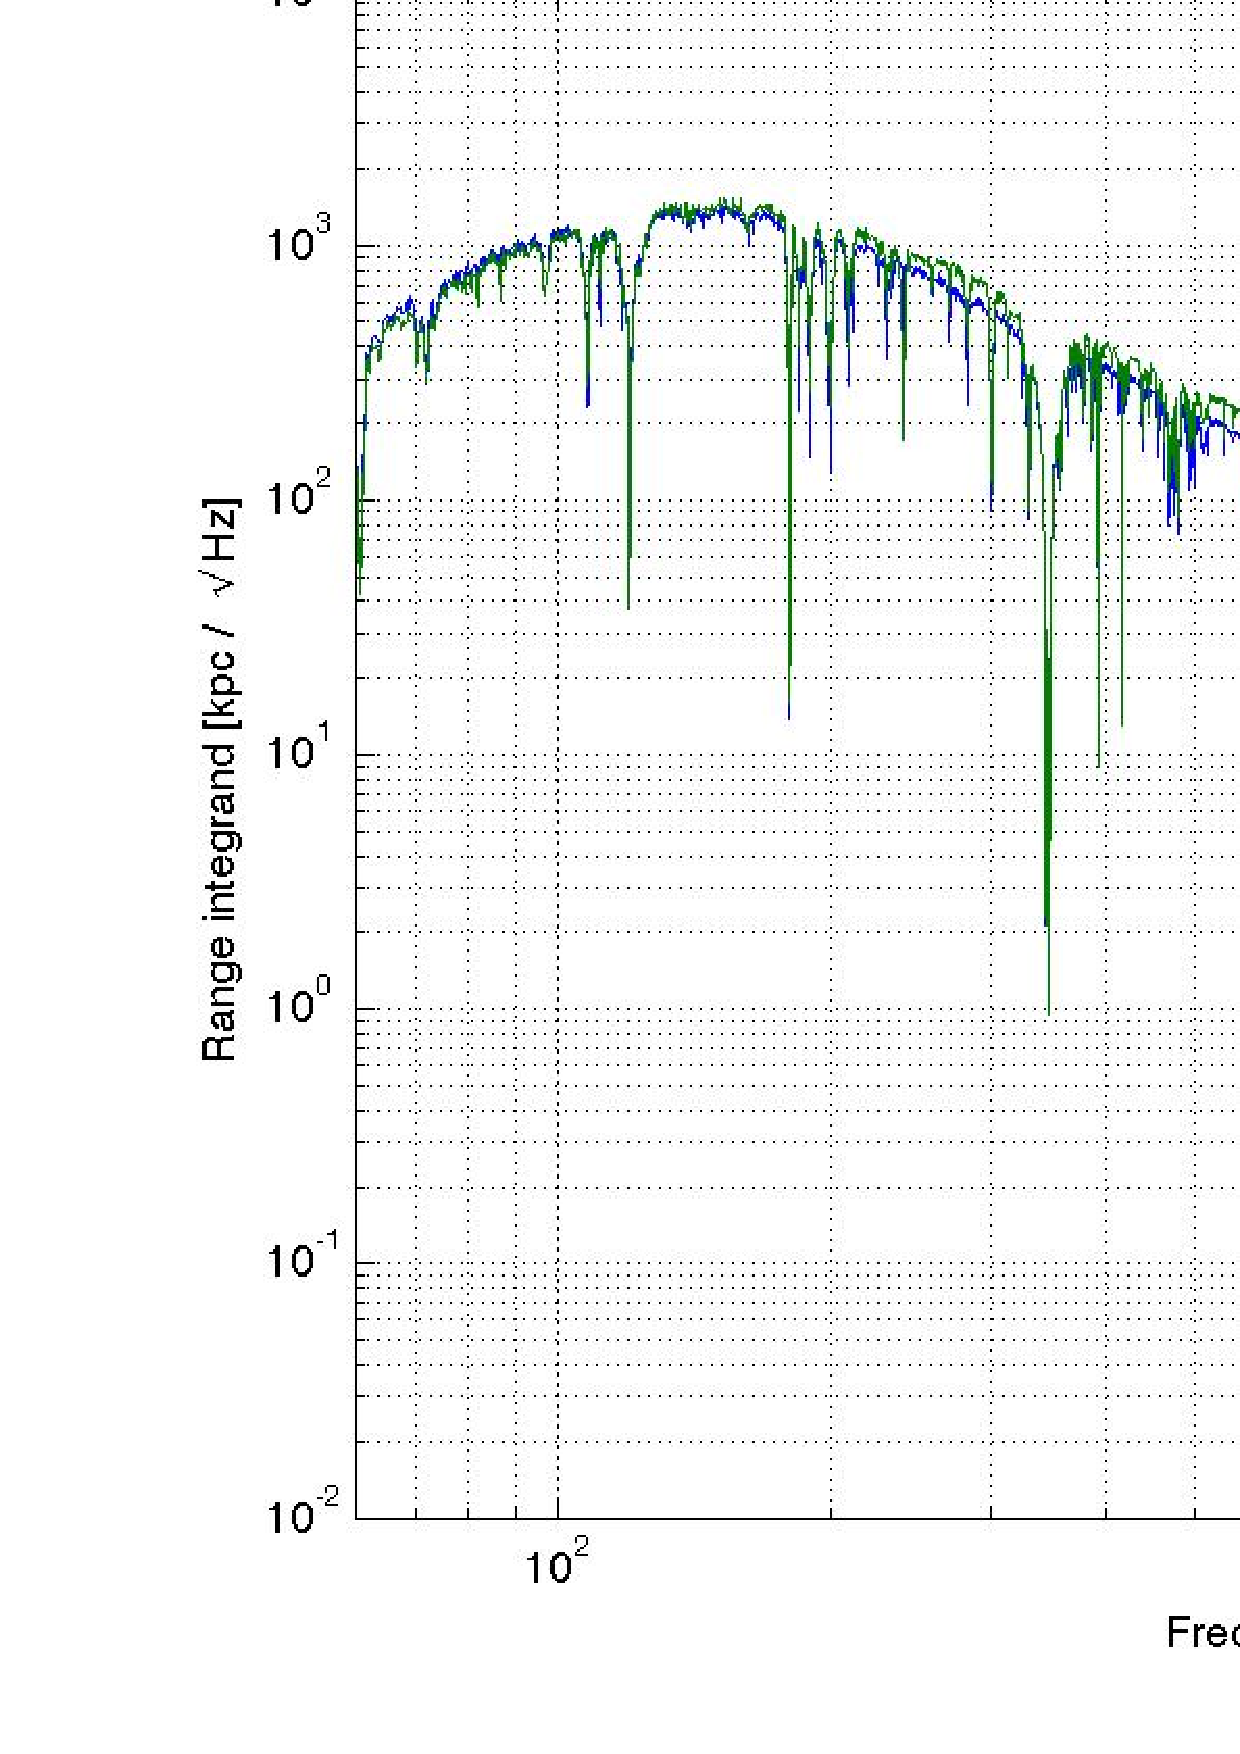
\includegraphics[width=0.45\paperwidth,height=0.45\paperheight,keepaspectratio]{range_integrand.jpeg}\protect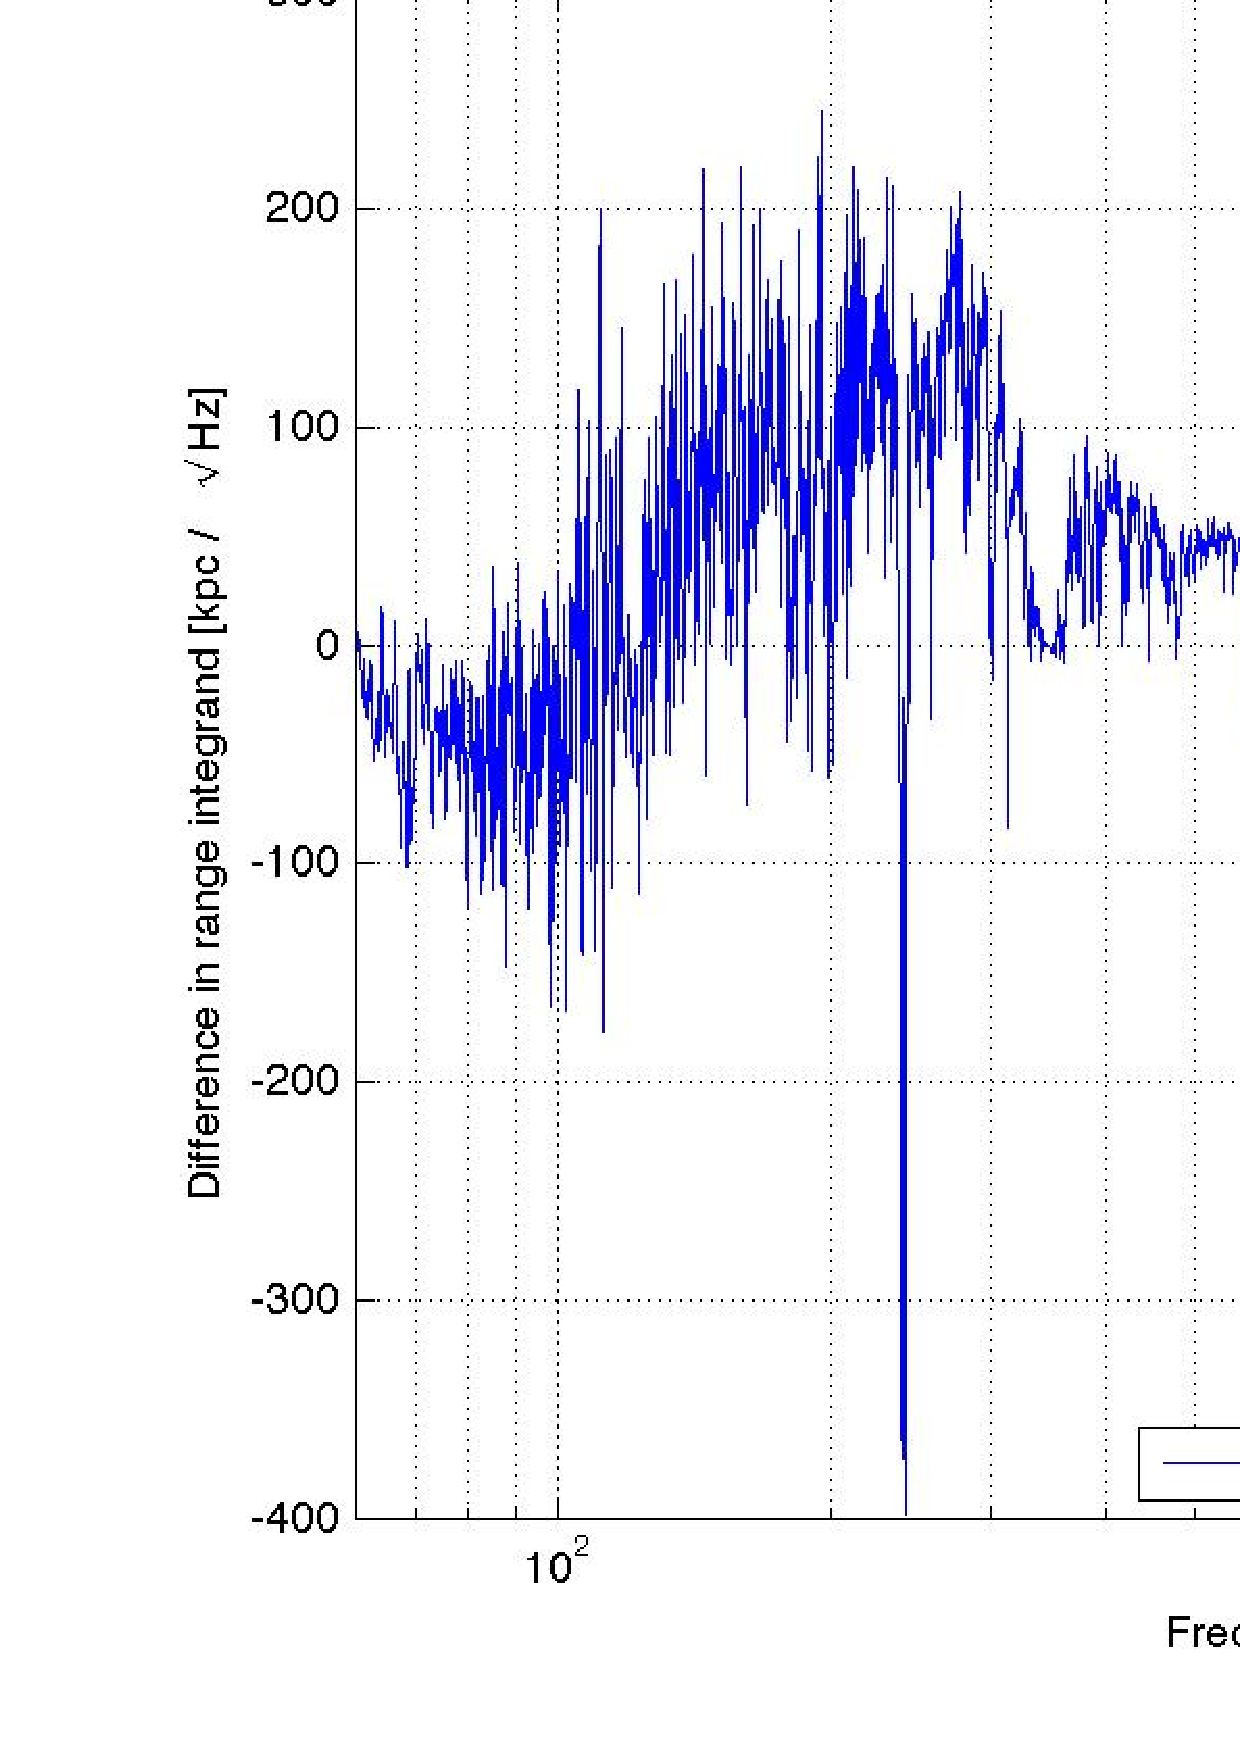
\includegraphics[width=0.45\paperwidth,height=0.45\paperheight,keepaspectratio]{range_integrand_difference.jpeg}}
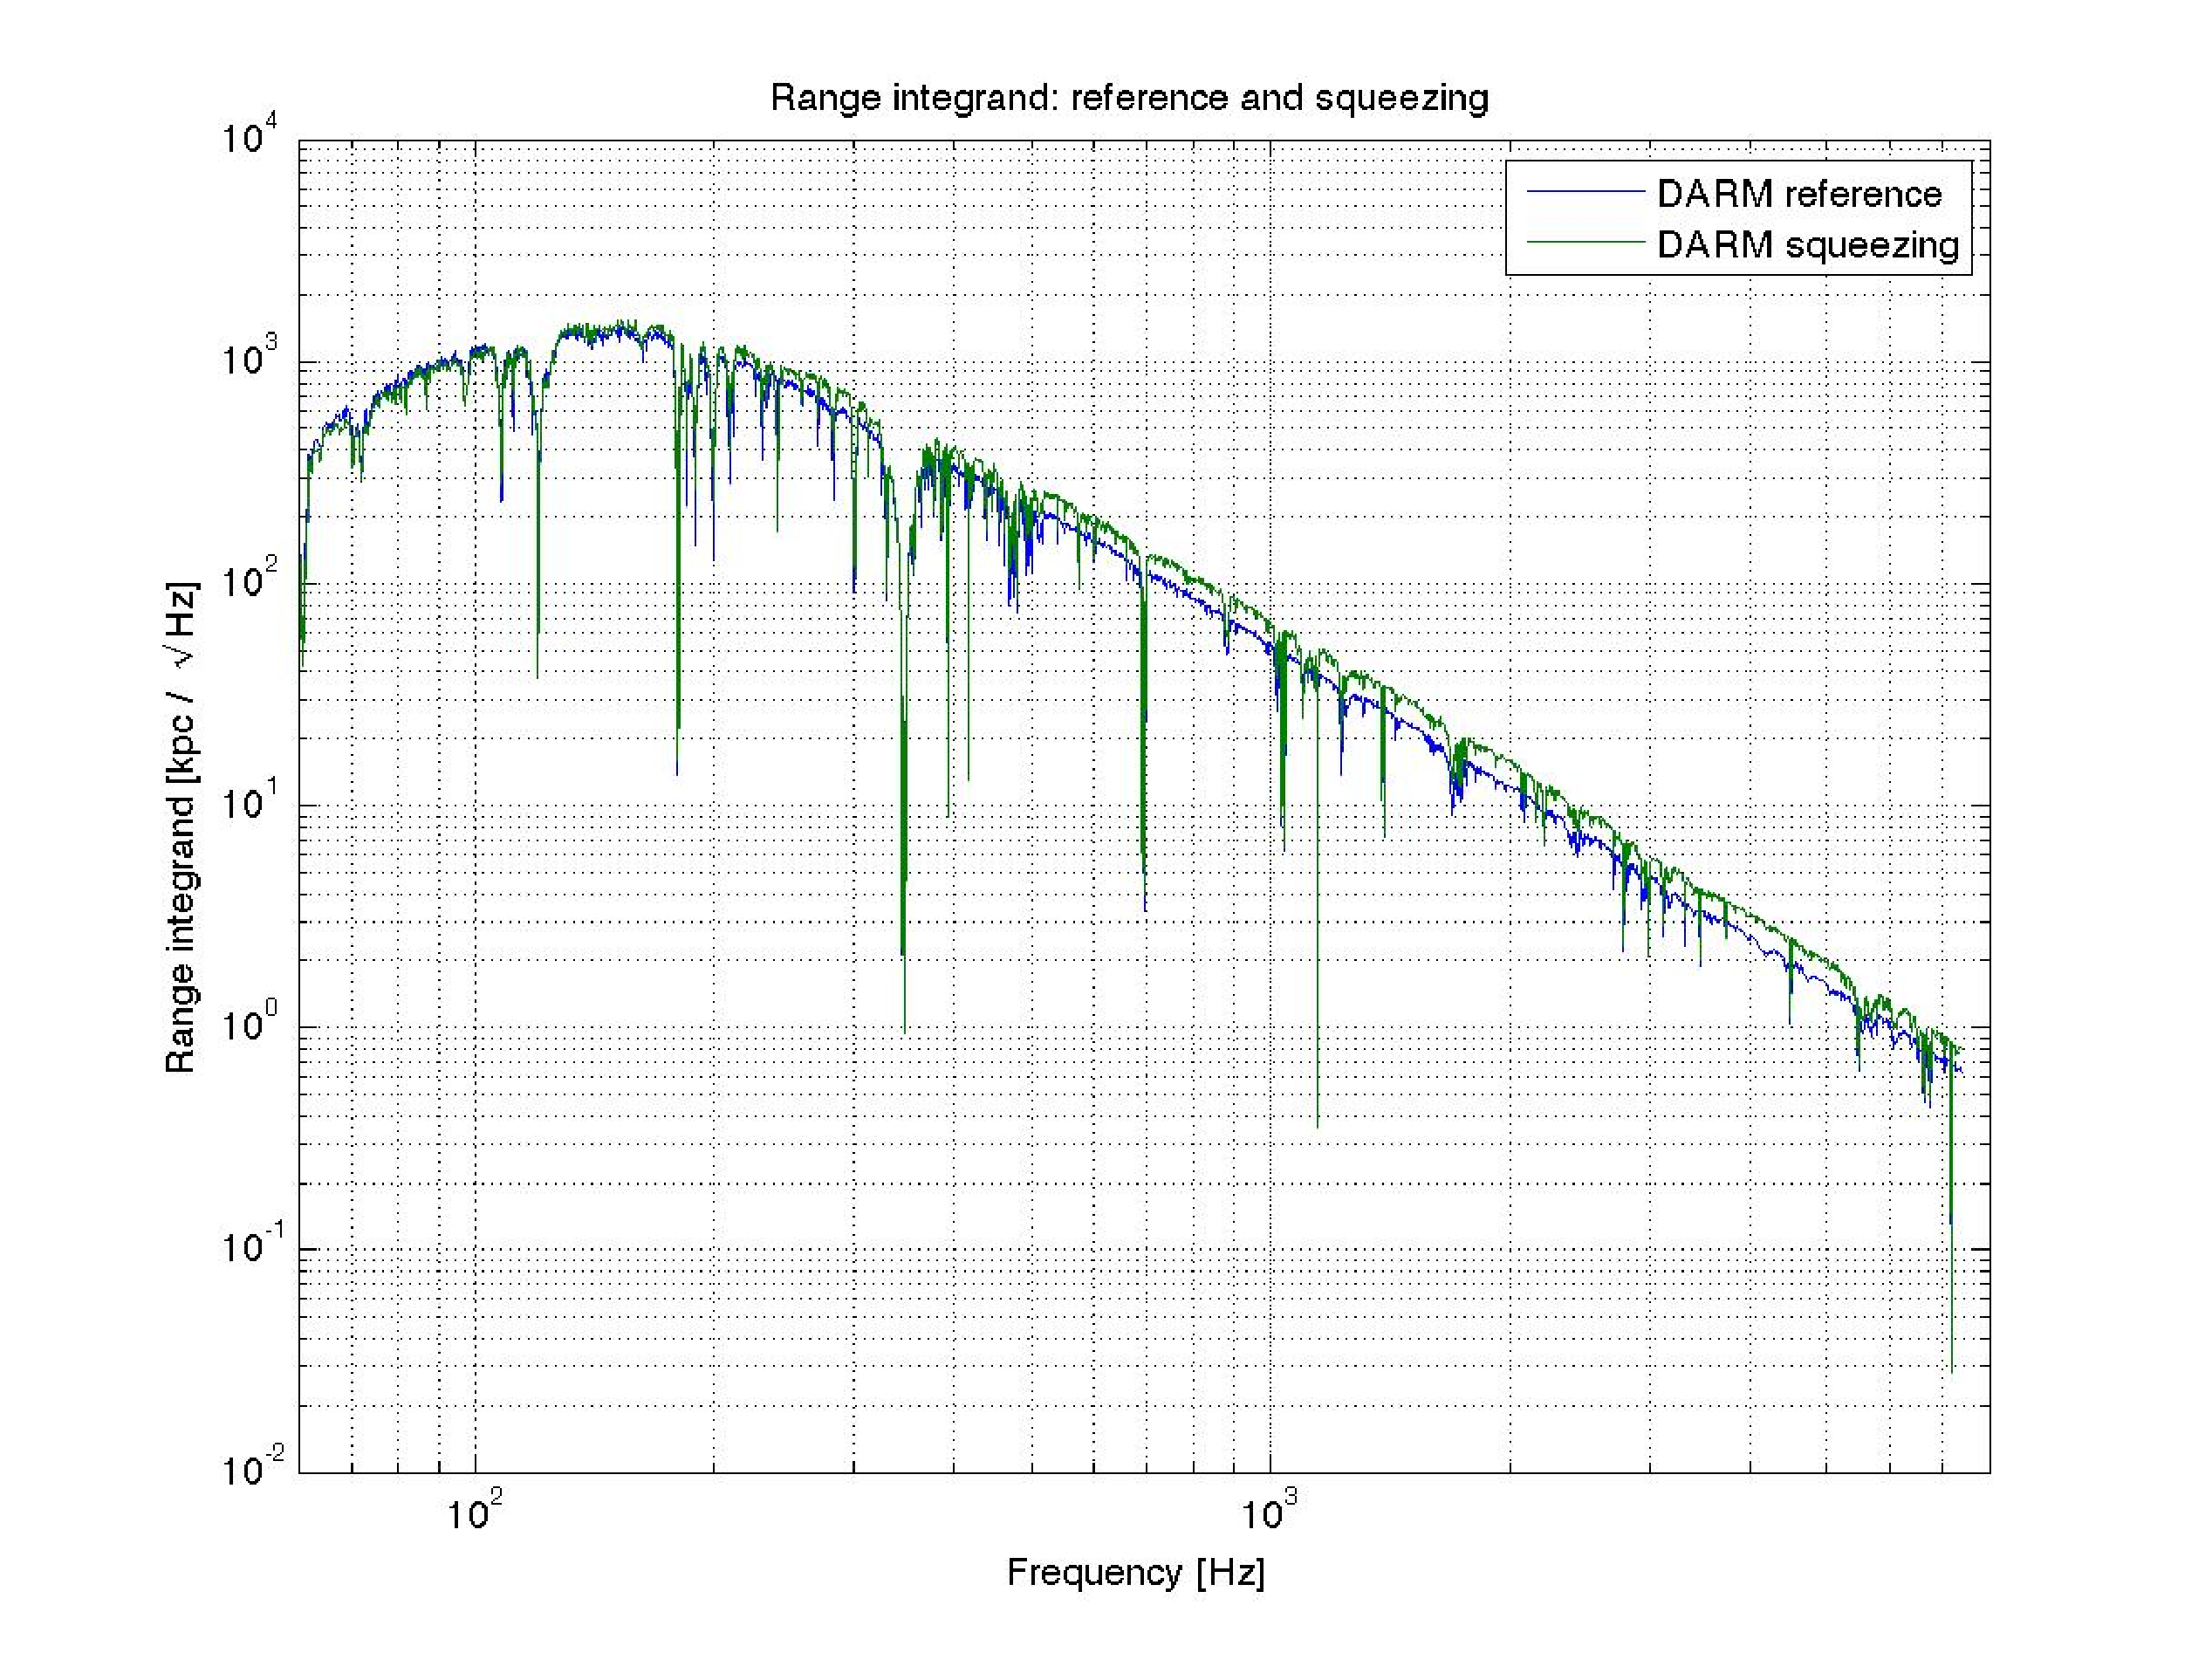
\includegraphics[height=0.5\paperheight, width=0.5\paperwidth,keepaspectratio]{range_integrand.eps}
\caption{Integrand of inspiral range as a function of frequency, with and without squeezing.}
\end{center}
\end{figure}
\begin{figure}
\begin{center}
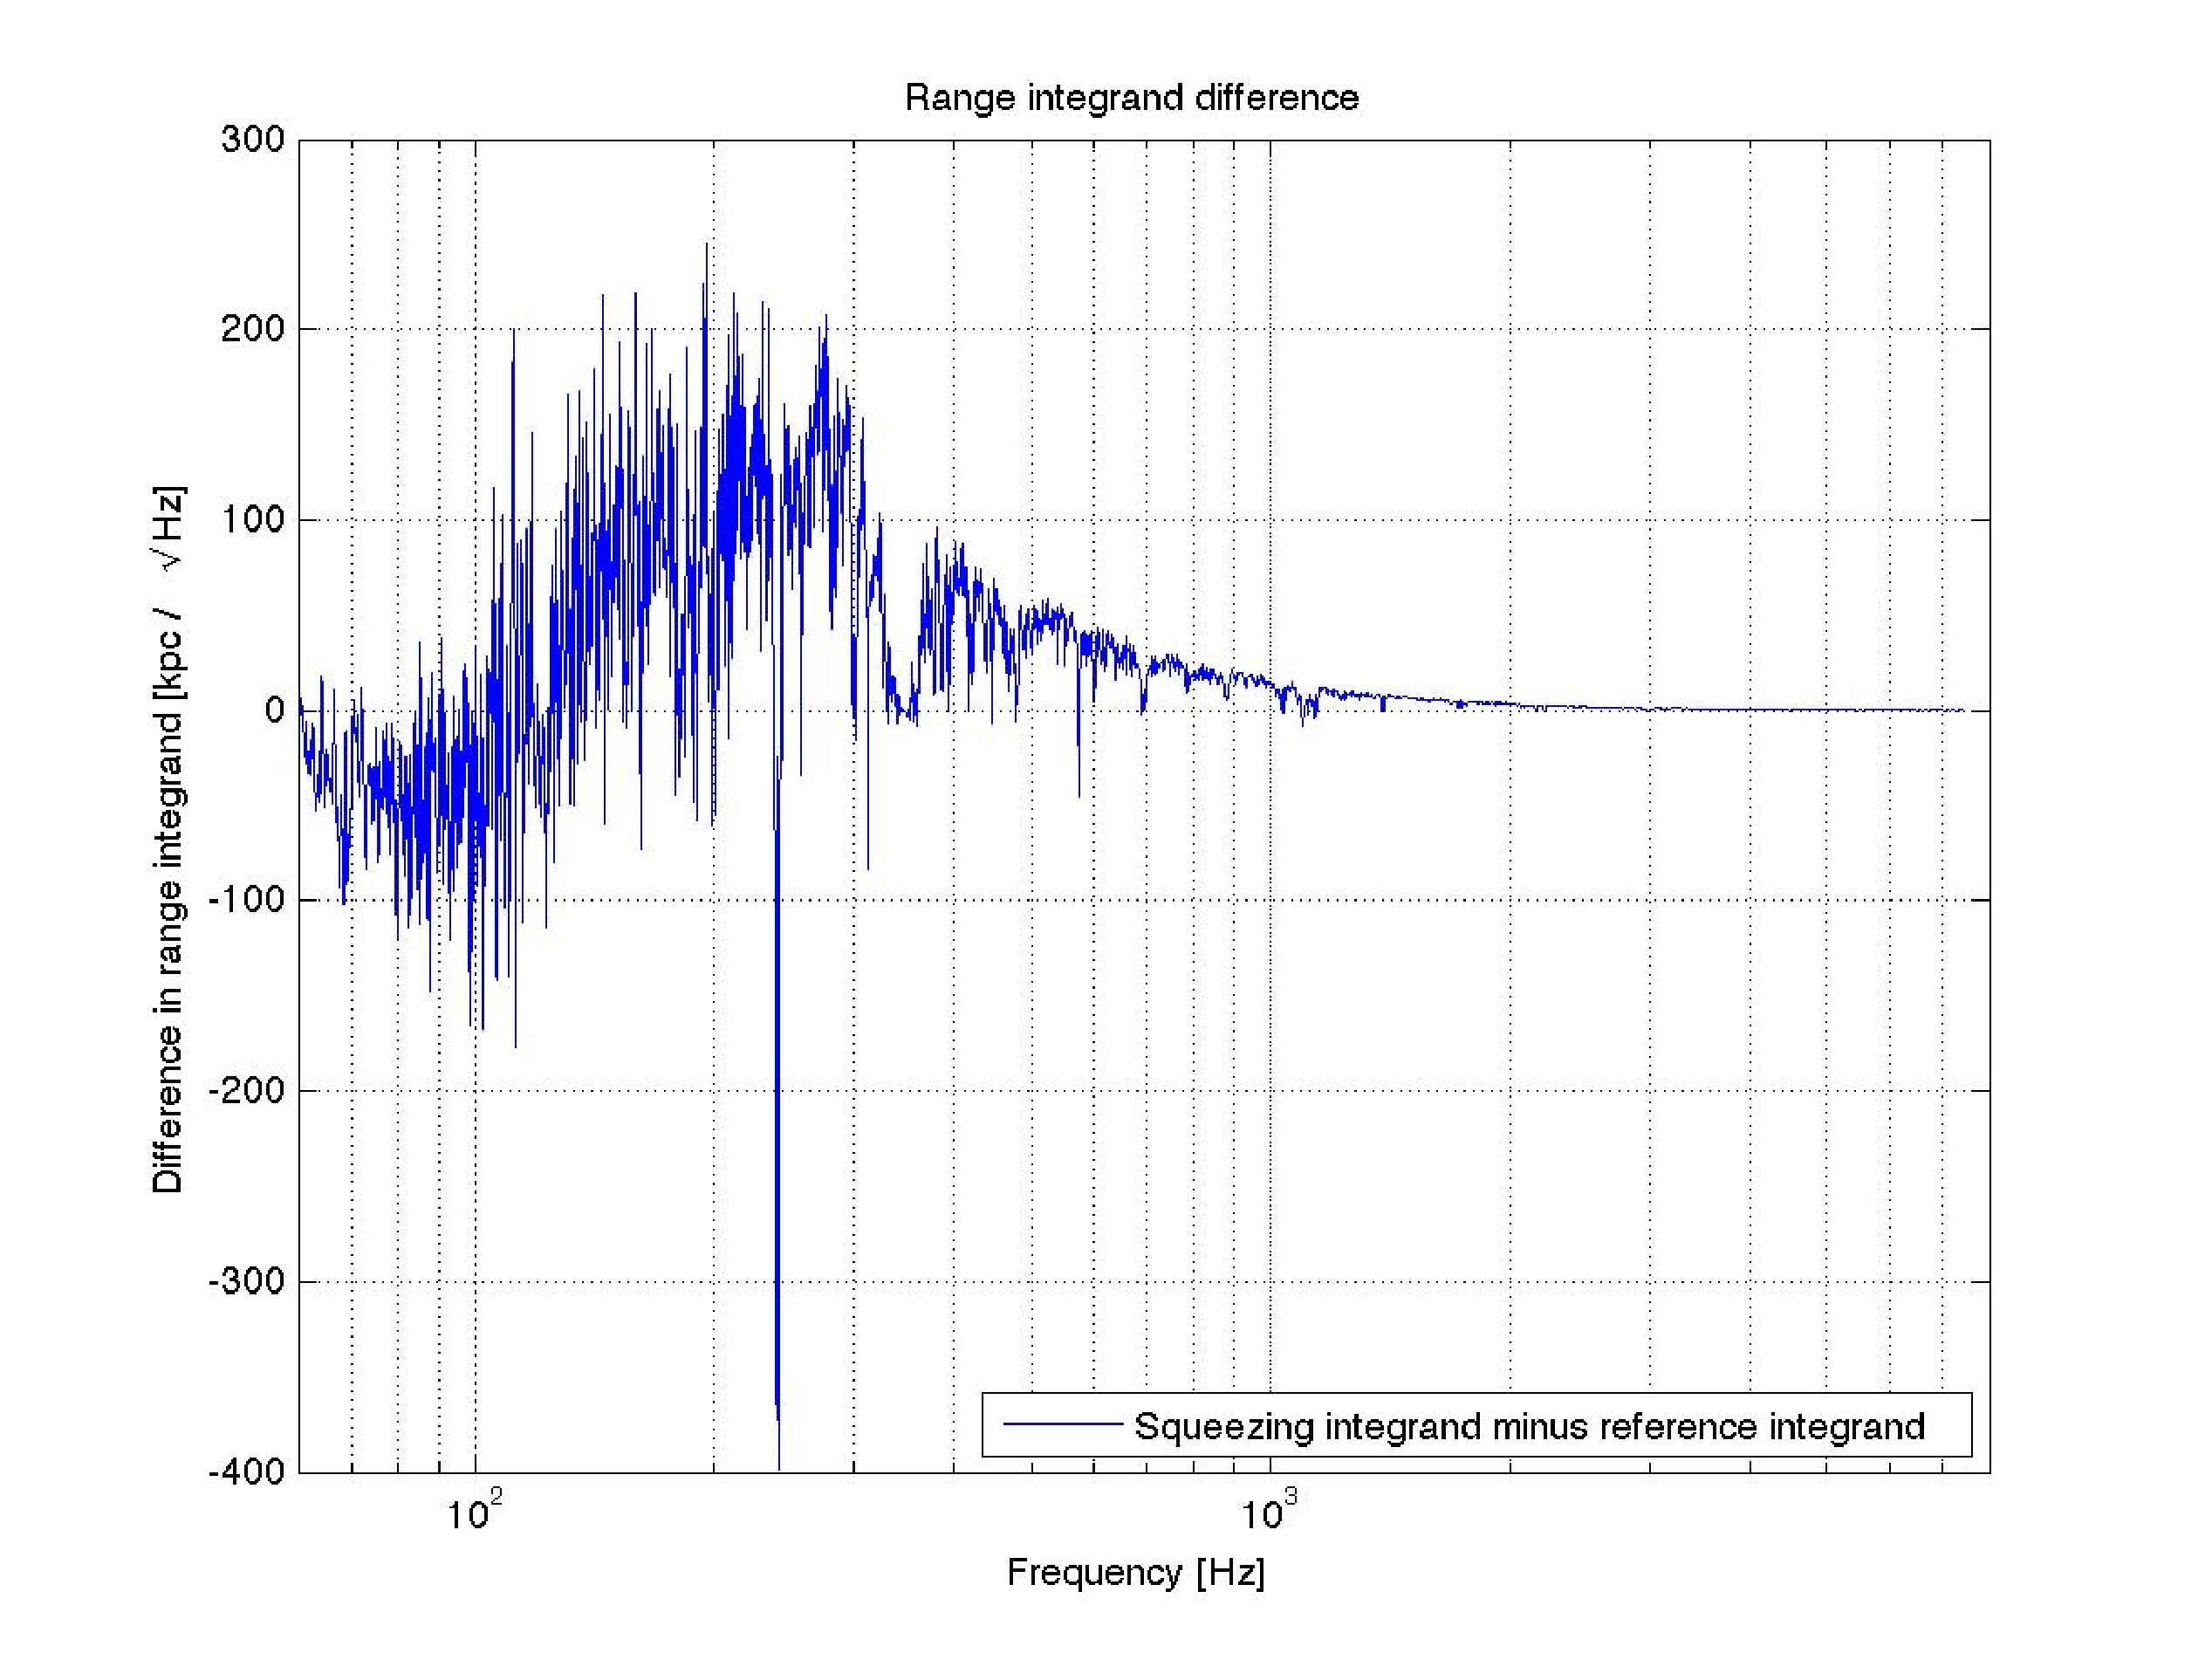
\includegraphics[height=0.5\paperheight, width=0.5\paperwidth,keepaspectratio]{range_integrand_difference.eps}
\caption{Net effect of squeezing on inspiral range integrand. Scientific benefit from squeezing is evident at the few hundred Hz `bucket' where initial LIGO is most sensitive, and although low frequency noise is slightly worse, this in an already noisy spectral band. Enhanced LIGO unambigiously benefitted from squeezing, proving the technique's efficacy.
}
\end{center}
\end{figure}




            \subsubsection{Figures of merit: inspiral range}
            \label{range_est}

                Range estimation after squeezing

		From the improved shot noise, we can see that squeezing at high frequencies bought enhanced LIGO a megaparsec of inspiral range. This number is impressive in several respects: our goal was to acheive a squeezing factor of perhaps as much as 3 dB, but to do it in the shot noise-limited region, at high frequencies, where the inspiral range equations (MATH: add the inspiral range equation if not already shown for feedforward!) count for much less. Morever, that range figure reflects the acheivement of squeezing down to 150 Hz, which is the lowest yet achieved for a gravitational wave interferometer, as can be seen in the Nature Photonics paper~\cite{BarsottiNatureSqueezing}


\section{Squeezing large interferometers}

        \subsection{Success and Advanced LIGO prospects}
        \label{squeezing_success}
            Results and hopes for aLIGO+ squeezing.

	    The squeezer group has a paper pending in review for Nature, written by Lisa Barsotti, in which we discuss our acheivement of perhaps 2 dB worth of squeezing (need to cite and check whether it is OK to use this number)~\cite{BarsottiNatureSqueezing}. It builds on the previous success of GEO600 in squeezing~\cite{GEO600NatureSqueezing}.

	    Discuss Sheila Dwyer's~\cite{DwyerPhaseNoise} and Sheon Chua's~\cite{ChuaBackscatteredLight} papers, since I am an author on both of them. We have a preliminary understanding now of at least two major problems: the quadrature phase noise fluctatuations and backscattered light. Backscattered light can be resolved in several ways. Phase noise must be progressively improved, as Sheila discusses, because we can hope to acheive the mature filter cavity design proposed below.

Discuss Lisa Barsotti's talk about the future prospect for LIGO using filter cavities, work that Tomoki Isogai is doing. With filter cavities, we can acheive frequency-dependent squeezing, having the best of both works by reducing quantum radiation pressure noise at low frequencies and shot noise at high, by using the filter cavity to produce a squeezed vacuum with a squeeze angle that varies as a function of frequency. Though as yet this filter cavity has yet to be constructed, it is in the works at MIT.

% Everything below is imported from my AEI talk




%\end{frame}

%\begin{frame}{Squeezing summary}
\subsection{Squeezing summary}

\begin{description}
\item [{Instrumental}] experience with technique important beyond Advanced
LIGO
\item [{Physical}] way to improve broad band of LIGO, benefit many searches
\item [{Illustrates}] need for best sensitivity at few hundred Hz
\item [{Question}] what can we improve \emph{post-facto?}
\end{description}
%\end{frame}


%        -------------------------------- 
%
%	The following is an example of using the commands \textit{ref}
%	and \textit{label}. With these commands theorems, chapters,
%	sections and figurres can be labeld with names in the tex file
%	and then refered to by these names in later tex files. In
%	chapter~\ref{intro} we saw section~\ref{sample_section} or
%	theorem~\ref{sample_theorem}.
%
%	Lastly, here is how to include a figure. First generate an
%	encapsulated postscript file in xfig, adobe illustrator or
%	some other program. The specific commands are found in
%	\textit{chap2.tex}.
%
%        \begin{figure}[htb]
%        \centerline{ \epsfig{figure=sample.eps, 
%        height =  1.5 in}}
%        \caption{Sample Figure}
%        \label{sample_figure}
%        \end{figure}

